\documentclass[a4paper, oneside]{thesis}

\usepackage[utf8]{inputenc}
\usepackage[T1]{fontenc}

%for including full pdf pages
\usepackage[]{pdfpages} 

%%%%%%%%%%%%%%%%%%%%%%%%%%%%%%%%%%%%%%%%%%%%%%%%%%%%%%%%%%%%%%%%%%%%%%%%%%%%%%%%%%%%%%%%%%%%%%%%%
% DOCUMENT METADATA

\title{A computer-based learning environment aimed for students at the 3rd and 4th grade level}
\thesistype{Bachelor's Thesis}

\author{Florian Bütler}
\email{flbuetle@ethz.ch}

\institute{Chair of Information Technology and Education \\[2pt]
ETH Zürich}

\supervisors{Prof.\ Juraj Hromkovič}

% Optionally, keywords and categories of the work can be shown (on the Abstract page)
%\keywords{Keywords go here.}
%\categories{ACM categories go here.}

\date{\today}

%%%%%%%%%%%%%%%%%%%%%%%%%%%%%%%%%%%%%%%%%%%%%%%%%%%%%%%%%%%%%%%%%%%%%%%%%%%%%%%%%%%%%%%%%%%%%%%%%

\begin{document}

\frontmatter % do not remove this line
\maketitle

\cleardoublepage

\begin{acknowledgements}
	prof hrom kovic

team of abz for feedback

proofreaders

\TODO{}
\end{acknowledgements}


\begin{abstract}
	a brief introduction describing the discipline that the paper belongs to
a clear and concise statement of your problem
a brief explanation of your solution and its key ideas
a brief description of the results obtained and their impacts
\end{abstract}

\tableofcontents

\mainmatter % do not remove this line

% Start writing here
\chapter{Introduction}

\section{Motivation and Background}

With the introduction of Lehrplan 21 Computer Science became an integral part of the Swiss education curriculum \cite{Lehrplan21}. Pupils learn to understand the basic concepts of Computer Science and how to use them for problem solving. These concepts include methods on how to process, evaluate and summarize data, how to securely communicate and how to develop solution strategies for simple problems of information processing \cite{MedienUndInformatik}. The Education and Counselling Center for Computer Science Education at ETH Zürich \cite{ABZ} supports schools to teach these concepts among others by providing teaching resources and learning environments.

\section{Goals}

The main goal in this bachelor thesis is to implement tasks and riddles based on the textbook “einfach Informatik 3/4”, that will be published in spring 2021 \cite{EinfachInformatik}, in a computer-based learning environment that teaches the following concepts:

\begin{itemize}
    \item representing information with symbols,
    \item keeping information secret and
    \item learning from data
\end{itemize}

for pupils in the second cycle i.e the third and fourth grade of elementary school.
Along with solving tasks and riddles about the mentioned topics the ability of reading, writing, counting and calculating is trained as well.

\section{Related Work}

\TODO{maybe: about other learning environments}

\section{Outline}

This report start with the architecture of the computer based learning environment and its core implementation. Next it dedicates a chapter to each of the aforementioned concepts. Each chapter explains first how the concept is thought by hands-on exercises, then it gives an in-depth technical insight on how these exercises are implemented. At this point it is needed to be mentioned that the shown code might be simplified to highlight the intersting aspects, improve readability and to keep this report consise. Testing and Continous integration of the project is discussed before, finally, the report ends with a conclusion of the project.

\chapter{Objective}
\chapter{Implementation}

\section{Introduction}

\section{Vue.js}

\section{Typescript}

\section{Basic functionality}

% basic functionality: click, drag&drop, undo, trashcan, difficulty, check, next
% tutorial with video
% styling like highlighting, locked
% game component and interface for games

\section{Representing Information with Symbols}

% words generating
% number systems

\section{Keeping Information Secret}

% drawing on canvas

\section{Learning from Data}

% sudoku solver

\section{Testing}

\subsection{Unit and Snapshot Testing}

% jest

\subsection{End to End Testing}

% nightwatch

\section{Continous Integration}

% gitlab CI

\chapter{Conclusion}
\label{chapter:conclusion}

The main goal in this bachelor thesis was to implement tasks and riddles based on the textbook “einfach Informatik 3/4” in a computer-based learning environment for pupils in the second cycle. The concepts covered in this thesis are:

\begin{itemize}
    \item representing information with symbols,
    \item keeping information secret and
    \item learning from data
\end{itemize}

\section{Obstacles}

framework: how to structure the code 

\section{Limitation}

An interesting aspect of this thesis was to implement so many different exercises teaching different concepts. However, since not all exercises of each topic in the textbook “einfach Informatik 3/4” were implemented, I consider this as a major drawback. Some exercises like \nameref{section:similarWords} are preparatory exercises for more advanced exercises like communication with damaged messages. For the next time I thing it would improve the overall learning experience of pupils if a whole topic is covered and not only a fraction of it.

\TODO{maybe also: own learning environment}

\section{Future Work}

The future work is directly derivated from its limitations.

A big imporovement would be to cover the remaining fraction of the exercises that were not covered in this learning environment. Especially, those that are build on exercises already implemented in this learning environment.

\TODO{maybe: integrate into existing learning environment}


% This displays the bibliography for all cited external documents. 
% All references have to be defined in the file references.bib and can then be cited from within this document.
\bibliographystyle{IEEEtran}
\bibliography{references}

% This creates an appendix chapter, comment if not needed.
\appendix
\chapter{First Chapter Title}

Lorem ipsum dolor sit amet, consetetur sadipscing elitr, sed diam nonumy
eirmod tempor invidunt ut labore et dolore magna aliquyam erat, sed diam
voluptua.\TODO{This is a TODO annotation.}

\section{First Section Title}

Lorem ipsum dolor sit amet, consetetur sadipscing elitr, sed diam nonumy
eirmod tempor invidunt ut labore et dolore magna aliquyam erat, sed diam
voluptua.

\subsection{First Subsection Title}

Lorem ipsum dolor sit amet, consetetur sadipscing elitr, sed diam nonumy
eirmod tempor invidunt ut labore et dolore magna aliquyam erat, sed diam
voluptua.\REMARK{This is a REMARK annotation.}

\begin{theorem}[First Theorem] \label{thm:first theorem} This is our first
theorem. \end{theorem}

\begin{proof} And this is the proof of the first theorem with a complicated
formula and a reference to Theorem \ref{thm:first theorem}. Lorem ipsum dolor
sit amet, consetetur sadipscing elitr, sed diam nonumy eirmod tempor invidunt
ut labore et dolore magna aliquyam erat, sed diam voluptua. Lorem ipsum dolor
sit amet, consetetur sadipscing elitr, sed diam nonumy eirmod tempor invidunt
ut labore et dolore magna aliquyam erat, sed diam voluptua. \begin{equation}
{\frac {\mathrm d}{\mathrm dx}}\arctan(\sin({x}^{2}))=-2 \cdot {\frac
{\cos({x}^{2})x}{-2+\left (\cos({x}^{2})\right )^{2}}} \end{equation}
\end{proof}

\begin{lemma} lorem ipsum dolor sit amet \end{lemma}

\begin{corollary} lorem ipsum dolor sit amet \end{corollary}

\begin{observation} lorem ipsum dolor sit amet \end{observation}

\begin{definition} lorem ipsum dolor sit amet \end{definition}

\begin{problem} lorem ipsum dolor sit amet \end{problem}

\begin{assumption} lorem ipsum dolor sit amet \end{assumption}

\begin{example} lorem ipsum dolor sit amet \end{example}

\begin{claim} lorem ipsum dolor sit amet \end{claim}

\begin{remark} lorem ipsum dolor sit amet \end{remark}

Note that in \LaTeX, ``quotes'' do not use the usual double quote characters.

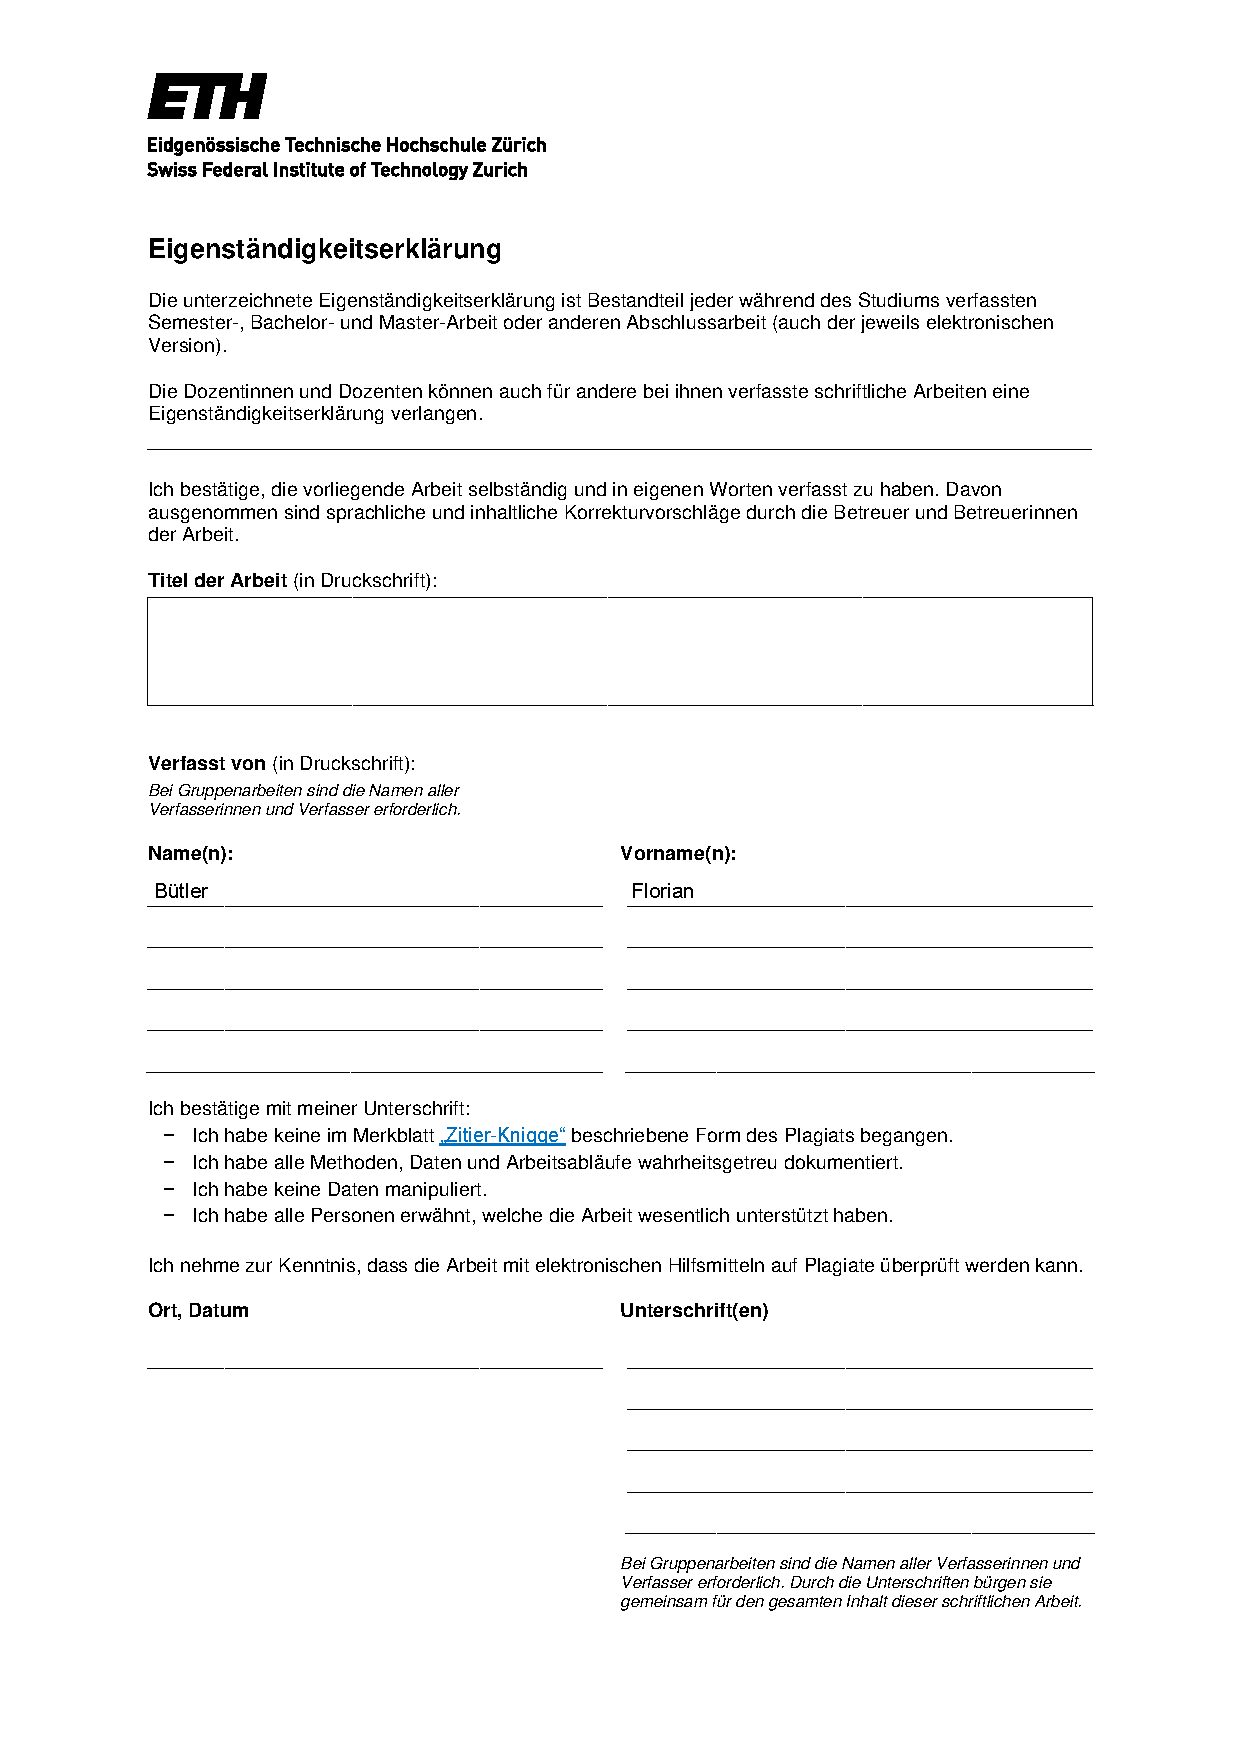
\includepdf[pages={1-},scale=1]{pdf/originality.pdf}

\end{document}